\documentclass[11pt,a4paper]{ivoa}
\usepackage[margin=4.25cm]{geometry} 
\input tthdefs
\setcounter{tocdepth}{2}

\title{WCS Transform Model}

% see ivoatexDoc for what group names to use here
\ivoagroup{Data Model Working Group}

\author{Mark Cresitello-Dittmar}
\author{David Berry}
\author{Steven Crawford}
\author{Nadia Dencheva}
\author{Tim Jenness}
\author{Omar Laurino}
\author{Stuart Mumford}
\author{Arnold Rots}
\author{Erik Tollerud}

%\author[????URL????]{????Alfred Usher Thor????}
%\author{????Fred Offline????}

\editor{Mark Cresitello-Dittmar}
\editor{Arnold Rots}

% \previousversion[????URL????]{????Funny Label????}
\previousversion{This is the first public release}
       
\newpage
\begin{document}

\begin{abstract}
  In creating version 2 of ``\emph{Space-Time Coordinate Metadata for the Virtual Observatory}'' (STC) \citep{std:STC} Data Model, it was decided to split the content into various component models which focus on particular aspects of the previous model scope.  
  
  This model covers the WCS Transform component, and includes the following concepts:
  \begin{itemize}
  \item The description of mathematical operations which form the building blocks for conversions from one coordinate space to another.
  \item The combination of individual operations into an arbitrarily complex Transform.
  \end{itemize}
\end{abstract}

\section*{Acknowledgments}
TBD: Get appropriate acknowledgment text

\section*{Conformance-related definitions}

The words ``MUST'', ``SHALL'', ``SHOULD'', ``MAY'', ``RECOMMENDED'', and
``OPTIONAL'' (in upper or lower case) used in this document are to be
interpreted as described in IETF standard RFC2119 \citep{std:RFC2119}.

The \emph{Virtual Observatory (VO)} is a
general term for a collection of federated resources that can be used
to conduct astronomical research, education, and outreach.
The \href{http://www.ivoa.net}{International
Virtual Observatory Alliance (IVOA)} is a global
collaboration of separately funded projects to develop standards and
infrastructure that enable VO applications.

\newgeometry{left=1.0in,right=1.0in,bottom=1.0in}
\section{Introduction}

\subsection{Motivation}
In Astronomy, it is common practice to define the relation between two coordinate spaces via a series of mathematical operations.  
With this relation, one can transform coordinates and other objects from one space to the other by applying these operations on
the set of points from the originating space.  This model describes these operations and the mechanisms for combining them.

\subsection{Context and Scope}
This document is a result of updating the ``\emph{Space-Time Coordinate Metadata for the Virtual Observatory}'' (STC) \citep{std:STC} model for use in VO-DML compliant models.

The update and revision of the STC model has sub-divided the content into component 
models, each covering a portion of the scope of the original model.  This has 
allowed for a better description of the relations between the various components, 
allows for independent development of the component models, and creates smaller, 
more digestible content for users.

This document covers the WCS Transforms model, including:
\begin{itemize}
  \item The description of mathematical operations which form the building blocks for conversions from one coordinate space to another.
  \item The combination of individual operations into an arbitrarily complex Transform.
\end{itemize}

The scope of this version of the model covers a core set of transform operations commonly used by the community.
It is designed to be compatible with FITS WCS metadata transport, and existing implementations
such as AST \citep{soft:AST}, GWCS \citep{soft:GWCS}, and wcslib \citep{soft:WCSLIB}.
It forms a foundation which can be built upon in future versions.

It is worth mentioning that this version of the model does NOT cover:
\begin{itemize}
  \item Spatial frame transformations (e.g. equatorial - galactic )
  \item Equivalent property transforms (e.g. Energy - Wavelength - Frequency )
  \item Time representations transforms (e.g. Date - MJD )
  \item Time transforms described in FITS WCS Paper IV.
\end{itemize}


\section{Use Cases and Requirements}
\label{sect:ucreq}

\subsection{Use Cases}
\label{sect:usecases}

\subsubsection{Cube model support}
\label{uc:Cube-model-support}

\begin{itemize}
\item Image axes \\
  Pixelated image axes are defined in a binned coordinate space with integerized values (pixel indexes).  However, 
  to be scientifically useful, we must map these pixel coordinates to one or more coordinate spaces with physical 
  meaning.  For example, we may transform them to various detector coordinates, or to an energy scale.  Ultimately, in 
  the spatial domain, we want the image axes represented in some celestial world coordinate system.  We note the following
  characteristics of mappings commonly found in astronomical image data:

  \begin{itemize}
    \item any combination of pixel axes may be involved in the transform to any given 'physical' space
    \item any pixel axis may be involved in more than one mapping
    \item mappings often involve multiple steps executed in sequence
    \item mappings may define a progressive migration in coordinate space (e.g. pixel - ccd - detector - sky - wcs )
    \item this progression may be given with explicitly defined intermediate coordinate spaces, or 
          as a single multi-stage transform.  It is, therefore, necessary that the Transform model facilitate the stacking of 
          operations in series.
    \item transform operations should be flexible in covering the n-dimensional space. e.g. the application of Scale operations to 1D, 2D, nD axes.
    \item pixel axis mappings are typically to a continuous domain, but may also be to a discrete domain such as Polarization state. 
  \end{itemize}

  Astronomical image cubes may have any number of dimensions, but are typically separable into co-dependent axes of 
  1,2, or 3 dimensions.  For example, a 4D image cube may contain a 1D spectral axis, 2D spatial axes, and 1D polarization axis.
  \begin{itemize}
    \item axes involved in a mapping need not be associated with the same physical domain.  e.g. X,Y = Map(x,y,temp); Transform with both spatial and thermal dependence.
    \item dimensionality may change between operations.
    \item this model must facilitate the combination of operations to cover an n-dimensional space from building blocks of commonly used operations. 
  \end{itemize}
      
  The industry standard for projections are defined in:
  \begin{itemize}
    \item Representations of celestial coordinates in FITS (paper II)\citep{WCSpaperII}
    \item Representations of spectral coordinates in FITS (paper III)\citep{WCSpaperIII}
  \end{itemize}
  This document, in no way, duplicates that work, but rather, defines model elements compatible with these specifications.  In that way,
  any implementation of these standards is automatically compatible with this model.  However, these standards do not cover the full
  range of non-linear distortions seen from today's instruments.  It is, therefore, necessary that this model be extensible to represent
  additional distortion types as needed.

\item Virtual data \\
  In addition to image axes, astronomical data is often defined as a mathematical function of other data.  In this case, the originating
  coordinate system is not pixelated, but any arbitrary coordinate space.  Examples of this include sparse cubes where the world coordinates
  are defined in terms of the physical detector coordinates, and image data values which may also have transforms associated with them.

\end{itemize}

\subsubsection{Transform workflow}
\label{uc:Transform-workflow}

  An implementation project focused on the Transform model being conducted by members of various facilities to evaluate the usability and applicability of the model to their missions.  The focus of this project is to exercise the Transform model through a workflow consisting of:
  \begin{itemize}
    \item serialization in YAML of various Transform operation sequences
    \item the generation and passing thereof between two Transform library implementations: AST and GWCS
  \end{itemize}
  This use case emphasizes the workflow and combination of atomic operations.
  \begin{itemize}
    \item combining operations in parallel to cover the dimension space
    \item combining operations in series to accomplish multi-stage mappings
    \item management and direction of axes through the operation sequence
    \begin{itemize}
      \item duplicate axes $x,y$ to send the pair into 2D-Polynomial transforms, producing $x',y'$
      \item from 4D axis set, send axes 1 and 3 into operation A, axis 2 into operation B, axis 4 into operation C.
      \item send 2D axis set into 3D operation, adding axis 3 with default value
    \end{itemize}
    \item handling of both forward and inverse operations
    \begin{itemize}
      \item for operations with no natural inverse, must have option to assign an independent operation to use in that direction.
    \end{itemize}
  \end{itemize}


\subsection{Requirements}
\label{sect:reqs}

 Examination and implementation of the above cases leads to a set of requirements distributed through the various STC component models.  Here we 
itemize those relevant to the transform model specifically.

\subsubsection{General}
Requirements pertaining to the overall criteria that the model must satisfy.
  \begin{itemize}
    \item [\textbf{[vodml.001]:}] The model shall be vo-dml compliant
    \item [\textbf{[vodml.002]:}] shall re-use, or refer to, dependent models for objects and concepts already defined in other models
    \item [\textbf{[vodml.003]:}] shall produce a validated vo-dml XML description
    \item [\textbf{[vodml.004]:}] shall produce documentation in vo-dml HTML format
    \item [\textbf{[vodml.005]:}] shall produce documentation in standard PDF format
  \end{itemize}

\subsubsection{Application/Usage}
Requirements pertaining to the user experience.  Note, as a data model, users will not typically interact directly with the model,
  \begin{itemize}
    \item [\textbf{[user.001]:}] Users should be able to identify and use basic content with minimal specialized information. 
      In other words, a generic utility should be able to find and use core elements without knowing a lot about the various extensions and uses of those elements.
    \item [\textbf{[user.002]:}] When applicable, the model should support usability by simplifying common scenarios. i.e. common things simple, complex things possible
    \item [\textbf{[user.003]:}] The model shall be easily extended to accommodate cases and applications not yet considered.
  \end{itemize}

\subsubsection{Content}
Requirements pertaining to the elements to be defined by the model.
\begin{itemize}

  \item [\textbf{[trans.001]:}] Shall facilitate the relation of two coordinate spaces through a mathematical formula (Transforms)
  \item [\textbf{[trans.002]:}] Shall define a set of atomic Transform operations commonly used in astronomical applications
  \begin{itemize}
    \item [\textbf{[trans.002.1]:}] at a minimum, shall accomodate common operations found in FITS images and data cubes, including but not limited to:
                 Linear, Matrix, FITS WCS projection, Lookup table, Polynomial (1D and 2D) 
    \item [\textbf{[trans.002.2]:}] shall accommodate and be compatible with established implementation packages AST, and GWCS 
  \end{itemize}
  \item [\textbf{[trans.003]:}] Shall allow the combination of operations in sequence, to form complex, multi-stage transforms.
  \item [\textbf{[trans.004]:}] Shall allow the combination of operations in parallel to cover the appropriate domain space
  \item [\textbf{[trans.005]:}] Shall support bi-directional workflow (forward and inverse), including the explicit assignment of independent operations for types which have no natural inverse.
  \item [\textbf{[trans.006]:}] Shall provide operations to facilitate a work flow that requires manipulation of the dimensional axes through the process
  \begin{itemize}
    \item [\textbf{[trans.006.1]:}] duplicate axes, e.g. to send axis pair (x,y) into 2 Poly2D operations to form (x',y')
    \item [\textbf{[trans.006.2]:}] shuffle axis order [x,y,z] => [x,z,y]
    \item [\textbf{[trans.006.3]:}] add or drop dimensions 
    \item [\textbf{[trans.006.4]:}] allows explicit control of flow in both forward and inverse directions
    \item [\textbf{[trans.006.4.1]:}] preferential selection of source in reverse direction for duplicated input axes
    \item [\textbf{[trans.006.4.2]:}] one-to-one axis mappings are not, necessarily, bi-directional
  \end{itemize}
\end{itemize}


\pagebreak
\subsection{Role within the VO Architecture}

\begin{figure}[h]
\centering

% As of ivoatex 1.2, the architecture diagram is generated by ivoatex in
% SVG; copy ivoatex/archdiag-full.xml to archdiag.xml and throw out
% all lines not relevant to your standard.
% Notes don't generally need this.  If you don't copy archdiag.xml,
% you must remove archdiag.svg from FIGURES in the Makefile.

\includegraphics[width=0.9\textwidth]{role_diagram.pdf}
\caption{Architecture diagram for this document}
\label{fig:archdiag}
\end{figure}

Fig.~\ref{fig:archdiag} shows the role this document plays within the
IVOA architecture \citep{note:VOARCH}.

\subsection{Model Dependencies }
  
  % INSERT FIGURE HERE
  \begin{figure}[h]
  \begin{center}
    \includegraphics[width=3.0in]{diagrams/model_dependency.png}
    \caption{WCS Transform model dependencies}\label{fig:overview}
  \end{center}
  \end{figure}

This model depends loosly on the IVOA Coordinates model in that it references coordinate systems defined in that model.

% Main Body of the document, extracted from vo-dml/xml using vo-dml2ivoatex
% with some post-processing.. mainly in the sequencing of content for better readability.
% -------------------------------------------
% Items to substitute into the ivoatex document template.
%
%\ivoagroup{Data Model Working Group}

%\title{WCS Transform Model}


%\author{Arnold Rots}
    
%\author{Mark Cresitello-Dittmar}
    
%\author{David Berry}
    
%\author{Steven Crawford}
    
%\author{Nadia Dencheva}
    
%\author{Tim Jenness}
    
%\author{Omar Laurino}
    
%\author{Stuart Mumford}
    
%\author{Erik Tollerud}
    
%\previousversion{0.0}
      
% -------------------------------------------

\pagebreak
\section{Model: trans }
  
  % INSERT FIGURE HERE
  \begin{figure}[h]
  \begin{center}
    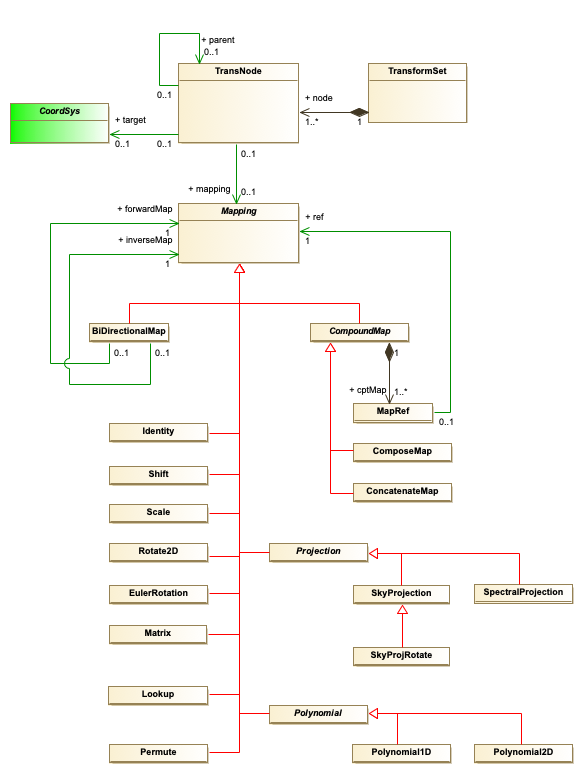
\includegraphics[width=5.25in]{diagrams/overview.png}
    \caption{Overview of WCS Transform model elements}\label{fig:overview}
  \end{center}
  \end{figure}

\pagebreak
  The transform model defines objects which can be used to construct expressions representing the relation between two coordinate systems. These may be used to transform coordinates and other objects defined in one coordinate system into corresponding objects in another coordinate system. There are two primary components to the model, the "Mapping", and the "TransformSet". 

  The "Mapping" object defines how to transform a set of "input" scalar values into a corresponding set of "output" scalar values. The Mapping supports transforms in either direction via "operations" which we refer to as the forward and inverse operations. The forward operation transforms the mapping inputs into mapping outputs. The inverse operation transforms the mapping outputs into mapping inputs. 

  The "TransformSet" object gives physical context to the "Mapping" by relating a parent coordinate system to a target coordinate system via a Mapping. The TransformSet model structure allows for the association of groups of inter-related coordinate systems. 

  Since a mapping expression can involve multiple steps between end points, we separate these features, such that the Mapping provides the path, and the TransformSet associates a Mapping with its source and target coordinate systems.

\pagebreak
\section{Mappings}
  % INSERT FIGURE HERE
  \begin{figure}[h]
  \begin{center}
    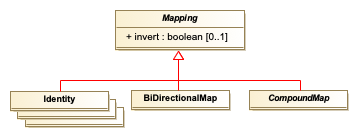
\includegraphics[width=3in]{diagrams/mappings_top.png}
    \caption{Top Level Mappings view}\label{fig:MapOps}
  \end{center}
  \end{figure}

  \subsection{Mapping (Abstract)}
  \label{sect:Mapping}
  The "Mapping" object defines how to transform a set of "input" scalar values into a corresponding set of "output" scalar values. The Mapping supports transforms in either direction via "operations" which we refer to here as the forward and inverse operations. The forward operation transforms the mapping inputs into mapping outputs. The inverse operation transforms the mapping outputs into mapping inputs. 

  There is possibility here for confusion regarding the meaning of the words "input" and "output". A clear distinction should be drawn between the inputs and outputs of a mapping and those of an operation. The inputs and outputs of a mapping are the same as the inputs and outputs of the mapping's forward operation, but are the reverse of the inputs and outputs of the mapping's inverse operation. Thus, the inputs of the inverse operation are the outputs of the mapping, etc. 

  \begin{figure}[h]
  \begin{center}
    \includegraphics[width=3in]{diagrams/mappings_flow.png}
  \end{center}
  \end{figure}

  Note, a mapping may in principle be inverted, but an operation cannot be inverted. Inverting a mapping means reversing the roles performed by its two operation - the original inverse operation is used as the new forward operation, and vice-versa. 

  We could support both forward and inverse operations by defining entirely separate expressions to describe the two transformations. However, that approach is bulky and requires more maintanence as any change to one object would require equivalent changes be made to the other. Since many operations have a natural inverse, a safer, more compact and flexible approach is to use a single object to describe both transformations. With this approach, a change to the one transform automatically applies to both directions. 

  This model leverages this compact approach, defining mappings with sufficient information to support both forward and inverse operations. Many mappings, such as shift, and rotation, have an analytical inverse, and both operations can be supported by a single set of parameters. For others, like polynomial, this is not true and so one of the two operations may be undefined. The BiDirectionalMap may be used to explicitely assign a different mapping for each direction. 

  In this model, we describe three flavors of mappings which allow specifications from very simple relations to arbitrarily complex relations built from a set of component mappings: 
  \begin{itemize}
  \item Atomic Mappings which perform a single arithmatic operation 
  \item BiDirectional Mapping with explicit specification of the mapping in the forward and inverse direction
  \item Compound Mappings which are used to control the workflow and build arbitrarily complex operations
  \end{itemize}

    \subsubsection{Mapping.invert}
      \textbf{vodml-id: Mapping.invert} \newline
      \textbf{type: \hyperref[sect:ivoa]{ivoa:boolean}} \newline
      \textbf{multiplicity: 0..1} \newline 
      Boolean flag indicates that the Mapping content defines its inverse operation rather than its forward operation and so the Mapping should be inverted before being used. In other words, the forward operation of the Mapping should be implemented using the inverse operation implied by the Mapping's contents, and vice versa. 

      For many operations, the inverse transformation can be directly derived from the forward transform. For instance, the inverse of a transform that simply adds a constant to each input is a transform of the same type, with a negated constant. However, there are potentially operations for which this cannot be done. For instance, the inverse of a transform that maps 3D Cartesian coordinates to spherical coordinates cannot be expressed by the same algorithm. This flag indicates that it should be used in its inverse sense. 

      In addition, the invert flag allows a complex compound transformation to be be inverted simply by toggling its invert flag. Without such a flag each component would need to be re-written to represent its inverse (if possible), and the order of serial transformations would need to be reversed - a much more complex and error prone process.


\pagebreak
\section{Atomic Mappings}

  % INSERT FIGURE HERE
  \begin{figure}[h]
  \begin{center}
    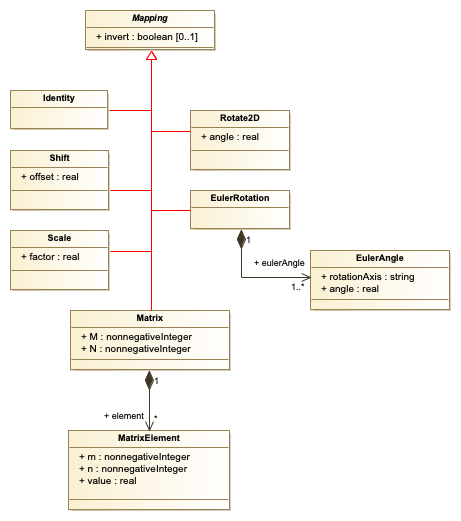
\includegraphics[width=3.75in]{diagrams/basic_operations.png}
    \caption{Arithmatic Transform Operations (partial)}\label{fig:basicOps}
  \end{center}
  \end{figure}

  Mappings which perform a single mathematical operation. As Mappings, these may be used in isolation for very simple relations, or used as components in more complex mapping expressions.

  \subsection{Identity}
  \label{sect:Identity}
    A 1-Dimensional operation which makes no change to the inputs. ( $x' = x$ )

  \subsection{Scale}
  \label{sect:Scale}
    A 1-Dimensional operator for simple scaling. ( $x' = factor \times x$ )

    \subsubsection{Scale.factor}
      \textbf{vodml-id: Scale.factor} \newline
      \textbf{type: \hyperref[sect:ivoa]{ivoa:real}} \newline
      \textbf{multiplicity: 1} \newline 
      The scale factor.

  \subsection{Shift}
  \label{sect:Shift}
    A 1-Dimensional operation defining a simple offset. ( $x' = x + offset$ )

    \subsubsection{Shift.offset}
      \textbf{vodml-id: Shift.offset} \newline
      \textbf{type: \hyperref[sect:ivoa]{ivoa:real}} \newline
      \textbf{multiplicity: 1} \newline 
      The amount of offset to apply.

  \subsection{Rotate2D}
  \label{sect:Rotate2D}
    A 2-Dimensional rotation operation.

    \subsubsection{Rotate2D.angle}
      \textbf{vodml-id: Rotate2D.angle} \newline
      \textbf{type: \hyperref[sect:ivoa]{ivoa:real}} \newline
      \textbf{multiplicity: 1} \newline 
      Rotation angle, in degrees, from the positive direction of axis 1 toward the positive direction of axis 2.

  \subsection{EulerRotation}
  \label{sect:EulerRotation}
    Defines a rotation operation in a 3-dimensional cartesian coordinate space, defined as a series of rotations about the native axes (x,y,z).

    \subsubsection{EulerRotation.eulerAngle}
      \textbf{vodml-id: EulerRotation.eulerAngle} \newline
      \textbf{type: \hyperref[sect:EulerAngle]{trans:EulerAngle}} \newline
      \textbf{multiplicity: 1..*} \newline 
      Rotation angle about a specified axis.

  \subsection{EulerAngle}
  \label{sect:EulerAngle}
    Angular rotation about a particular axis of a 3-dimensional cartesian coordinate space.

    \subsubsection{EulerAngle.rotationAxis}
      \textbf{vodml-id: EulerAngle.rotationAxis} \newline
      \textbf{type: \hyperref[sect:ivoa]{ivoa:string}} \newline
      \textbf{multiplicity: 1} \newline 
      Identifies the axis of rotation. MUST be 'x', 'y', or 'z'

    \subsubsection{EulerAngle.angle}
      \textbf{vodml-id: EulerAngle.angle} \newline
      \textbf{type: \hyperref[sect:ivoa]{ivoa:real}} \newline
      \textbf{multiplicity: 1} \newline 
      Angle of rotation, in degrees. Angle sign follows the right-hand rule, where positive values indicate clockwise rotation (looking in +axis direction), negative values for counter-clockwise.

  \subsection{Matrix}
  \label{sect:Matrix}
    An M x N matrix operation. Each cell of the matrix is provided by a MatrixElement object. Missing elements should be considered to equal 0.

    \noindent \textbf{constraint} \newline
    \indent    \textbf{detail:} Matrix.element maxlength = M*N \newline


    \subsubsection{Matrix.M}
      \textbf{vodml-id: Matrix.M} \newline
      \textbf{type: \hyperref[sect:ivoa]{ivoa:nonnegativeInteger}} \newline
      \textbf{multiplicity: 1} \newline 
      Number of rows in the matrix.

    \subsubsection{Matrix.N}
      \textbf{vodml-id: Matrix.N} \newline
      \textbf{type: \hyperref[sect:ivoa]{ivoa:nonnegativeInteger}} \newline
      \textbf{multiplicity: 1} \newline 
      Number of columns in the matrix.

    \subsubsection{Matrix.element}
      \textbf{vodml-id: Matrix.element} \newline
      \textbf{type: \hyperref[sect:MatrixElement]{trans:MatrixElement}} \newline
      \textbf{multiplicity: 0..*} \newline 
      Collection of MatrixElements which define each cell of the matrix. The total number of elements MUST NOT exceed M*N, any missing elements result in a cell with value=0.0.

  \subsection{MatrixElement}
  \label{sect:MatrixElement}
    The value of cell m,n in an M x N matrix.

    \subsubsection{MatrixElement.m}
      \textbf{vodml-id: MatrixElement.m} \newline
      \textbf{type: \hyperref[sect:ivoa]{ivoa:nonnegativeInteger}} \newline
      \textbf{multiplicity: 1} \newline 
      Matrix cell row number.

    \subsubsection{MatrixElement.n}
      \textbf{vodml-id: MatrixElement.n} \newline
      \textbf{type: \hyperref[sect:ivoa]{ivoa:nonnegativeInteger}} \newline
      \textbf{multiplicity: 1} \newline 
      Matrix cell column number.

    \subsubsection{MatrixElement.value}
      \textbf{vodml-id: MatrixElement.value} \newline
      \textbf{type: \hyperref[sect:ivoa]{ivoa:real}} \newline
      \textbf{multiplicity: 1} \newline 
      Matrix cell value.

  \subsection{Projection (Abstract)}
  \label{sect:Projection}

    % INSERT FIGURE HERE
    \begin{figure}[h]
    \begin{center}
      \includegraphics[width=5.25in]{diagrams/fitswcs_operations.png}
      \caption{FITS WCS Transform Operations}\label{fig:WCSOps}
    \end{center}
    \end{figure}

    Abstract head of World Coordinate System (WCS) projection operations. We do not attempt to define the operations here, but instead, provide extensions which support the transforms described in the FITS WCS papers II and III.

    \subsubsection{Projection.param}
      \textbf{vodml-id: Projection.param} \newline
      \textbf{type: \hyperref[sect:ProjectionParam]{trans:ProjectionParam}} \newline
      \textbf{multiplicity: 0..*} \newline 
      Set of 0 or more parameters providing supplemental metadata required to execute a particular projection algorithm. The number and meaning of the parameters depends on the algorithm. They are typically in the from of keyword/value pairs, so we provide a simple ProjectionParam element to accommodate these. The detailed content description is left to the WCS paper.

  \subsection{ProjectionParam}
  \label{sect:ProjectionParam}
    Simple parameter specification for WCS Projections. The parameter is modeled as a simple name/value pair. The details of expectations for the various projection algorithms is left to the WCS paper describing the algorithm.

    \subsubsection{ProjectionParam.name}
      \textbf{vodml-id: ProjectionParam.name} \newline
      \textbf{type: \hyperref[sect:ivoa]{ivoa:string}} \newline
      \textbf{multiplicity: 1} \newline 
      The parameter name as described in the WCS papers for each operation type.

    \subsubsection{ProjectionParam.value}
      \textbf{vodml-id: ProjectionParam.value} \newline
      \textbf{type: \hyperref[sect:ivoa]{ivoa:real}} \newline
      \textbf{multiplicity: 1} \newline 
      The value for the parameter.

  \subsection{SkyProjection}
  \label{sect:SkyProjection}
    This class corresponds to the Spherical Projection component of the FITS WCS paper II. As in the paper, this operation describes the mapping from the intermediate \&quot;Projection Plane\&quot; to the \&quot;Native Spherical\&quot; coordinate system. This model supports all defined projection types, where the appropriate code is specified in the algorithm attribute. All projection parameters are to be provided through the ProjectionParam list according to the descriptions given in the FITS WCS paper.

    \subsubsection{SkyProjection.algorithm}
      \textbf{vodml-id: SkyProjection.algorithm} \newline
      \textbf{type: \hyperref[sect:SkyProjectionType]{trans:SkyProjectionType}} \newline
      \textbf{multiplicity: 1} \newline 
      The projection algorithm to apply. The value MUST be taken from the enumeration of standard sky projection algorithms. Extracted from 'ctype' in the FITS WCS representations.

  \subsection{SkyProjRotate}
  \label{sect:SkyProjRotate}
    This class extends SkyProjection to include the Spherical Rotation component of the FITS WCS paper II. This operation describes the mapping from the "Native Spherical" coordinate system to the "Celestial" coordinate system. The reference values are provided at the appropriate attribute, while all other parameters (e.g. LONPOLE, LATPOLE) are to be provided through the ProjectionParam list according to the descriptions given in the FITS WCS paper.

    \subsubsection{SkyProjRotate.referenceValue}
      \textbf{vodml-id: SkyProjRotate.referenceValue} \newline
      \textbf{type: \hyperref[sect:ivoa]{ivoa:real}} \newline
      \textbf{multiplicity: 2} \newline 
      The target reference values in each dimension. Equivalent to 'crval' in FITS WCS representations.

  \subsection{SpectralProjection}
  \label{sect:SpectralProjection}
    This class represents a nonlinear one-dimensional spectral transform as detailed in the FITS WCS paper III.

    \subsubsection{SpectralProjection.referenceValue}
      \textbf{vodml-id: SpectralProjection.referenceValue} \newline
      \textbf{type: \hyperref[sect:ivoa]{ivoa:real}} \newline
      \textbf{multiplicity: 1} \newline 
      The target reference value for the axis. Equivalent to 'crval' in FITS WCS representations.

    \subsubsection{SpectralProjection.algorithm}
      \textbf{vodml-id: SpectralProjection.algorithm} \newline
      \textbf{type: \hyperref[sect:SpectralProjectionType]{trans:SpectralProjectionType}} \newline
      \textbf{multiplicity: 1} \newline 
      The projection algorithm to apply. The value MUST be taken from the enumeration of non-linear spectral projection algorithms. Extracted from 'ctype' in FITS WCS representations.

    \subsubsection{SpectralProjection.coordType}
      \textbf{vodml-id: SpectralProjection.coordType} \newline
      \textbf{type: \hyperref[sect:SpectralCoordType]{trans:SpectralCoordType}} \newline
      \textbf{multiplicity: 1} \newline 
      The resulting spectral coordinate type code. Values MUST be taken from the enumerated list of spectral coordinate types. Extracted from 'ctype' in FITS WCS representations.

  \subsection{Polynomial (Abstract)}
  \label{sect:Polynomial}
    % INSERT FIGURE HERE
    \begin{figure}[h]
    \begin{center}
      \includegraphics[width=3in]{diagrams/polynomial_operations.png}
      \caption{Polynomial Transform Operations}\label{fig:PolyOps}
    \end{center}
    \end{figure}

    Abstract head of a family of Polynomial distortion operations.

    \subsubsection{Polynomial.order}
      \textbf{vodml-id: Polynomial.order} \newline
      \textbf{type: \hyperref[sect:ivoa]{ivoa:nonnegativeInteger}} \newline
      \textbf{multiplicity: 1} \newline 
      The order, or degree, of the polynomial expression.

  \subsection{Polynomial1D}
  \label{sect:Polynomial1D}
    A 1-Dimensional Polynomial transform represented by the expression:
    \indent $x' = \sum_{i=0}^{order} c_i\times x^{i} $ \newline
    Each term is provided by a PolyCoeff1D object. Missing terms are considered to have a coefficient of 0.0.

    \subsubsection{Polynomial1D.term}
      \textbf{vodml-id: Polynomial1D.term} \newline
      \textbf{type: \hyperref[sect:PolyCoeff1D]{trans:PolyCoeff1D}} \newline
      \textbf{multiplicity: 1..*} \newline 
      A term in the polynomial expression.

  \subsection{PolyCoeff1D}
  \label{sect:PolyCoeff1D}
    A term of the polynomial expression. This object provides the coefficient (c) and power (p) of the term, forming the expression $c \times x^{p}$.

    \subsubsection{PolyCoeff1D.coeff}
      \textbf{vodml-id: PolyCoeff1D.coeff} \newline
      \textbf{type: \hyperref[sect:ivoa]{ivoa:real}} \newline
      \textbf{multiplicity: 1} \newline 
      Multiplicitive coefficient of the term.

    \subsubsection{PolyCoeff1D.power}
      \textbf{vodml-id: PolyCoeff1D.power} \newline
      \textbf{type: \hyperref[sect:ivoa]{ivoa:nonnegativeInteger}} \newline
      \textbf{multiplicity: 1} \newline 
      The power to raise the value for this term.

  \subsection{Polynomial2D}
  \label{sect:Polynomial2D}
    A 2-Dimensional Polynomial transform represented by the expression:
    \indent $x' = \sum_{i+j<=order} c_{ij}\times x^{i}\times y^{j}$ \newline
    Each term is provided by a PolyCoeff2D object. Missing terms are considered to have a coefficient of 0.0.

    \subsubsection{Polynomial2D.term}
      \textbf{vodml-id: Polynomial2D.term} \newline
      \textbf{type: \hyperref[sect:PolyCoeff2D]{trans:PolyCoeff2D}} \newline
      \textbf{multiplicity: 1..*} \newline 
      A term in the polynomial expression.

  \subsection{PolyCoeff2D}
  \label{sect:PolyCoeff2D}
    A term of the polynomial expression. This object provides the coefficient (c) and power (p) of the term, forming the expression $c \times x^{p[0]} \times y^{p[1]}$.

    \subsubsection{PolyCoeff2D.coeff}
      \textbf{vodml-id: PolyCoeff2D.coeff} \newline
      \textbf{type: \hyperref[sect:ivoa]{ivoa:real}} \newline
      \textbf{multiplicity: 1} \newline 
      Multiplicitive coefficient of the term.

    \subsubsection{PolyCoeff2D.power}
      \textbf{vodml-id: PolyCoeff2D.power} \newline
      \textbf{type: \hyperref[sect:ivoa]{ivoa:nonnegativeInteger}} \newline
      \textbf{multiplicity: 2} \newline 
      The power to raise the values for this term in each dimension.

  \subsection{Lookup}
  \label{sect:Lookup}

    % INSERT FIGURE HERE
    \begin{figure}[h]
    \begin{center}
      \includegraphics[width=4in]{diagrams/lookup_operations.png}
      \caption{Lookup Table Transform Operations}\label{fig:LookupOps}
    \end{center}
    \end{figure}

    Defines a lookup table operation. The Lookup is comprised of a series of value pairs (LookupEntry) which link specific points in the native system to corresponding points in the target system. The 'interpolation' flag tells the user how to interpret data which falls between entries in the lookup table. All members of the series MUST be of the same type. Lookup tables with StringEntry type content MUST have interpolation="None". 

    Handling Enumerated data: A common usage of a Lookup operation is to map image pixel index to an enumeration, such as a Polarization state. This can be handled by two means:
    \begin{enumerate}
    \item Define a numeric equivalent for each enumeration literal, and use NumericEntry types. Casting to the corresponding literal occurs outside of the operation. 
    \item Your local model can define a LookupEntry extension which maps the native value directly the target EnumerationLiteral. 
    \end{enumerate}
    The details of either approach for particular enumerations is considered outside the scope of this document.

    \subsubsection{Lookup.interpolation}
      \textbf{vodml-id: Lookup.interpolation} \newline
      \textbf{type: \hyperref[sect:InterpolationMethod]{trans:InterpolationMethod}} \newline
      \textbf{multiplicity: 0..1} \newline 
      Specifies the form of interpolation, if any, prescribed to be performed.

    \subsubsection{Lookup.bounds\_error}
      \textbf{vodml-id: Lookup.bounds\_error} \newline
      \textbf{type: \hyperref[sect:ivoa]{ivoa:boolean}} \newline
      \textbf{multiplicity: 0..1} \newline 
      Flag to specify behaviour outside the lookup table data bounds. True indicates an error condition, False indicates that the associated "fill" entry should be returned. If no "fill" entry is provided, the value should be extrapolated.

    \subsubsection{Lookup.entry}
      \textbf{vodml-id: Lookup.entry} \newline
      \textbf{type: \hyperref[sect:LookupEntry]{trans:LookupEntry}} \newline
      \textbf{multiplicity: 1..*  (ordered)} \newline 
      Set of lookup table entries forming a discrete mapping from the native space to the target space.

  \subsection{LookupEntry (Abstract)}
  \label{sect:LookupEntry}
    This is an abstract head of lookup table entry objects. Each entry provides a discrete translation of a 'native' value to the corresponding 'target' value.

    \subsubsection{LookupEntry.fill}
      \textbf{vodml-id: LookupEntry.fill} \newline
      \textbf{type: \hyperref[sect:ivoa]{ivoa:boolean}} \newline
      \textbf{multiplicity: 0..1} \newline 
      When TRUE, the entry provides values to be used outside the Lookup table data domain. MUST only appear first or last in the sequence. If missing, it is considered to be FALSE.

  \subsection{NumericEntry}
  \label{sect:NumericEntry}
    A 1-Dimensional discrete mapping of numeric values.

    \subsubsection{NumericEntry.nativeValue}
      \textbf{vodml-id: NumericEntry.nativeValue} \newline
      \textbf{type: \hyperref[sect:ivoa]{ivoa:real}} \newline
      \textbf{multiplicity: 1} \newline 
      The native, or reference, value of the lookup entry.

    \subsubsection{NumericEntry.targetValue}
      \textbf{vodml-id: NumericEntry.targetValue} \newline
      \textbf{type: \hyperref[sect:ivoa]{ivoa:real}} \newline
      \textbf{multiplicity: 1} \newline 
      The target, or resulting, value of the lookup entry.

  \subsection{NumericEntry2D}
  \label{sect:NumericEntry2D}
    A 2-Dimensional discrete mapping of numeric values.

    \subsubsection{NumericEntry2D.nativeValue}
      \textbf{vodml-id: NumericEntry2D.nativeValue} \newline
      \textbf{type: \hyperref[sect:ivoa]{ivoa:real}} \newline
      \textbf{multiplicity: 2} \newline 
      The native, or reference, value of the lookup entry.

    \subsubsection{NumericEntry2D.targetValue}
      \textbf{vodml-id: NumericEntry2D.targetValue} \newline
      \textbf{type: \hyperref[sect:ivoa]{ivoa:real}} \newline
      \textbf{multiplicity: 2} \newline 
      The target, or resulting, value of the lookup entry.

  \subsection{StringEntry}
  \label{sect:StringEntry}
    A 1-Dimensional discrete mapping of an integer counter to a corresponding string form. Since the result is non-numeric, a Lookup operation with StringEntry-s can only be used at the end of a Transform sequence.

    \subsubsection{StringEntry.nativeValue}
      \textbf{vodml-id: StringEntry.nativeValue} \newline
      \textbf{type: \hyperref[sect:ivoa]{ivoa:integer}} \newline
      \textbf{multiplicity: 1} \newline 
      The native, or reference, value of the lookup entry.

    \subsubsection{StringEntry.targetValue}
      \textbf{vodml-id: StringEntry.targetValue} \newline
      \textbf{type: \hyperref[sect:ivoa]{ivoa:string}} \newline
      \textbf{multiplicity: 1} \newline 
      The target, or resulting, value of the lookup entry.


  \subsection{Permute}
  \label{sect:Permute}
    % INSERT FIGURE HERE
    \begin{figure}[h]
    \begin{center}
      \includegraphics[width=2.0in]{diagrams/permute_operation.png}
      \caption{Permute Operation}\label{fig:PermuteOps}
    \end{center}
    \end{figure}
    Permute the order and possibly number of dimensions between operations. This operation facilitates the workflow through the operation sequence. It is comprised of an ordered axismap list defining the output axis sequence in terms of the source (input) axes. It supports the reorder, duplication, and dropping of dimensions. 
    \begin{itemize}
    \item[Reorder Example]: We have a 3-dimensional coordinate (x,y,z) and wish to perform a 2-dimensional transform on the (x,z) plane. Define a Permute operation to reorder the axes from (x,y,z) to (y,x,z) using an axismap list specifying the new axis order, [2,1,3]. The results feed into the next step ( 1D + 2D operations ). 
    \item[Duplicate Example]: We have 2-dimensional coordinate (x,y) feeding two Polynomial2D operations to form (x',y'). Define a Permute operation with axismap list specifying sourceAxis set [1,2,1,2]. The result feeds into the next step ( Polynomial2D + Polynomial2D operations). 
    \item[Drop Example]: We have a 5-dimensional input feeding into a 3x3 Matrix operation. Define a Permute operation selecting the relevant axis set [1,3,5], the remaining axes, [2,4], are dropped. 
    \item[Add Example]: We have a 2-dimensional operation feeding into axes [1,3] of a 3-dimensional operation. Define a Permute operation with numSourceAxes=2; and sourceAxis set [1,0,2] where output axis 2 also specifies the fixed seed value.
    \end{itemize}

    \subsubsection{Permute.numSourceAxes}
      \textbf{vodml-id: Permute.numSourceAxes} \newline
      \textbf{type: \hyperref[sect:ivoa]{ivoa:nonnegativeInteger}} \newline
      \textbf{multiplicity: 1} \newline 
      The number of input axes. Used to verify dimensional coverage in forward and inverse directions. For example, numSourceAxes=4 with axismap=[1,3] indicates that axes [2,4] have been dropped.

    \subsubsection{Permute.axismap}
      \textbf{vodml-id: Permute.axismap} \newline
      \textbf{type: \hyperref[sect:PermuteAxis]{trans:PermuteAxis}} \newline
      \textbf{multiplicity: 0..*  (ordered)} \newline 
      Ordered list defining the number and order of the resulting axis set. Each entry provides the source (input) dimension for that output dimension.

  \subsection{PermuteAxis}
  \label{sect:PermuteAxis}
    Entry for the Permute operation, this object defines the mapping of input dimension to output dimension. The output dimension is determined from its order in the axismap list.

    \subsubsection{PermuteAxis.sourceAxis}
      \textbf{vodml-id: PermuteAxis.sourceAxis} \newline
      \textbf{type: \hyperref[sect:ivoa]{ivoa:nonnegativeInteger}} \newline
      \textbf{multiplicity: 1} \newline 
      Source (input) dimension number, 1 based.

    \subsubsection{PermuteAxis.seedValue}
      \textbf{vodml-id: PermuteAxis.seedValue} \newline
      \textbf{type: \hyperref[sect:ivoa]{ivoa:real}} \newline
      \textbf{multiplicity: 0..1} \newline 
      Value to assign for the new dimensional axis.


\pagebreak
\section{BiDirectional Mappings}

  % INSERT FIGURE HERE
  \begin{figure}[h]
  \begin{center}
    \includegraphics[width=2.5in]{diagrams/bidirectional_map.png}
    \caption{Workflow Operations}\label{fig:BiDirMaps}
  \end{center}
  \end{figure}

  \subsection{BiDirectionalMap}
  \label{sect:BiDirectionalMap}
    The BiDirectionalMap supports cases where one wants to explicitely define independent transforms for the forward and inverse operations. This may be because a mapping does not have a natural inverse, or dictated by the requirements of the application. The associated mappings do not have to be of the same type. The forward operation of the BiDirectionalMap is supported by the forward operation of the forwardMap, and the inverse operation of the BiDirectionalMap by the inverse operation of the inverseMap.

  \begin{figure}[h]
  \begin{center}
    \includegraphics[width=2.5in]{diagrams/bidirectional_flow.png}
  \end{center}
  \end{figure}

 If the 'invert' flag is True, this is reversed so that the forward operation of the BiDirectionalMap is supported by the inverse operation of the inverseMap, and the inverse operation of the BiDirectionalMap by the forward operation of the forwardMap.

    \subsubsection{BiDirectionalMap.inverseMap}
      \textbf{vodml-id: BiDirectionalMap.inverseMap} \newline
      \textbf{type: \hyperref[sect:Mapping]{trans:Mapping}} \newline
      \textbf{multiplicity: 1} \newline 
      The Mapping that defines the inverse operation of the BiDirectionalMap. The inverse operation of the target Mapping is used as the inverse operation of the BiDirectionalMap. If the inverse operation of the target Mapping is undefined, then the inverse operation of the BiDirectionalMap is also undefined. The forward operation of the target Mapping is never used and may be undefined.

    \subsubsection{BiDirectionalMap.forwardMap}
      \textbf{vodml-id: BiDirectionalMap.forwardMap} \newline
      \textbf{type: \hyperref[sect:Mapping]{trans:Mapping}} \newline
      \textbf{multiplicity: 1} \newline 
      The Mapping that defines the foward operation of the BiDirectionalMap. The forward operation of the target Mapping is used as the foward operation of the BiDirectionalMap. If the forward operation of the target Mapping is undefined, then the forward operation of the BiDirectionalMap is also undefined. The inverse operation of the target Mapping is never used and need not be defined.


\pagebreak
\section{Compound Mappings}

  % INSERT FIGURE HERE
  \begin{figure}[h]
  \begin{center}
    \includegraphics[width=1.8in]{diagrams/workflow_operations.png}
    \caption{Workflow Operations}\label{fig:WorkOps}
  \end{center}
  \end{figure}

  \subsection{CompoundMap (Abstract)}
  \label{sect:CompoundMap}
    Abstract class to facilitate the combination of Mappings in various ways. Since they are themselves mappings, they can be used as a components in other compound mappings to create arbitrarily complex transform expressions.

    \subsubsection{CompoundMap.cptMap}
      \textbf{vodml-id: CompoundMap.cptMap} \newline
      \textbf{type: \hyperref[sect:MapRef]{trans:MapRef}} \newline
      \textbf{multiplicity: 1..*  (ordered)} \newline 
      List of component mappings. Joins multiple mappings together to form a single unit. The interpretation of the list set depends on the particular sub-class of CompoundMap.

  \subsection{ComposeMap}
  \label{sect:ComposeMap}
    Combines the component mappings in series. This allows the building of multi-stage transforms such as a Matrix operation followed by a WCS Projection. When the invert flag is 'True', the forward operation of the ComposeMap is defined by the inverse of the content, iterating the component list in reverse order, executing the inverse operation of each component.

  \subsection{ConcatenateMap}
  \label{sect:ConcatenateMap}
    Combines the component mappings in parallel. This enables the building of a mapping which covers the full dimension space of the input. Axes are distributed to the component mappings in order. For example, to perform a shift on a 2-dimensional coordinate (x,y), one would join two Shift maps giving the offset in x and y respectively. When the 'invert' flag is True, the forward operation of the ConcatenateMap is defined by applying the inverse operations of the component mappings.

  \subsection{MapRef}
  \label{sect:MapRef}
    An entry in the CompountMap component mapping list. Holds a reference to the component mapping.

    \subsubsection{MapRef.ref}
      \textbf{vodml-id: MapRef.ref} \newline
      \textbf{type: \hyperref[sect:Mapping]{trans:Mapping}} \newline
      \textbf{multiplicity: 1} \newline 
      Reference to the component Mapping.


\pagebreak
\section{Transforms}

  % INSERT FIGURE HERE
  \begin{figure}[h]
  \begin{center}
    \includegraphics[width=3.0in]{diagrams/transforms_top.png}
    \caption{Transforms}\label{fig:Transforms}
  \end{center}
  \end{figure}

  \subsection{TransformSet}
  \label{sect:TransformSet}
    TransformSet supports the relation of coordinate systems via Mappings. The design is such that it supports the relation of collections of related coordinates systems by the various mappings between them. 

    A single TransformSet can relate a tree of spatial coordinate systems, individual TransNodes can be used as the parent for multiple branches. For example:
    \begin{itemize}
    \item pixel - chip - tiled detector - detector - tangent plane 
    \item chip - chip physical 
    \item detector - mirror spherical 
    \item tangent plane - celestial 
    \end{itemize}

    Each transition is encapsulated by a TransNode instance linking the coordinate system of its parent TransNode to the target coordinate system (that of the TransNode) with a Mapping (from the parent to target systems). A simple transform from system A to system B requires two TransNodes, one describing system A (with no Mapping), and another describing system B with the Mapping from A to B.

    \subsubsection{TransformSet.node}
      \textbf{vodml-id: TransformSet.node} \newline
      \textbf{type: \hyperref[sect:TransNode]{trans:TransNode}} \newline
      \textbf{multiplicity: 1..*} \newline 
      A node in the transform set, relating a parent and target coordinate system with the corresponding mapping specification.

  \subsection{TransNode}
  \label{sect:TransNode}
    TransNode is a container object relating a parent coordinate system and a target coordinate system (that of the node) with the mapping relation between them. The associated Mapping MUST be constructed such that the mapping inputs correspond to the parent coordinate system and the mapping outputs to the target coordinate system. 

    If either the parent node or mapping is NULL, the other MUST also be NULL. This forms a 'root' node, containing only the target coordinate system, and serves as an origination node in the TransformSet. 

    If the target is NULL, the parent and mapping MUST NOT be NULL, additionally such a node MUST NOT be the end point of a node sequence (ie: must be the 'parent' of another node). This type of node can be useful for cases where the mapping defines the transform to an unspecified intermediate coordinate system, and enables a more efficient and compact structure for the TransformSet by forming a node at this intermediate coordinate system which can serve as the parent for multiple subsequent nodes.

    \subsubsection{TransNode.parent}
      \textbf{vodml-id: TransNode.parent} \newline
      \textbf{type: \hyperref[sect:TransNode]{trans:TransNode}} \newline
      \textbf{multiplicity: 0..1} \newline 
      This identifies the source coordinate system node. The associated mapping describes the transformation from this parent system to the target system of this node. Will be NULL for 'root' nodes.

    \subsubsection{TransNode.target}
      \textbf{vodml-id: TransNode.target} \newline
      \textbf{type: coords:CoordSys} \newline
      \textbf{multiplicity: 0..1} \newline 
      This identifies the target coordinate system node. It is the represenitive coordinate system for this node. The associated mapping describes the transformation from the parent system of this node to this target system. The coordinate systems themselves are described in the IVOA "Astronomical Coordinates and Coordinate Systems" model.

    \subsubsection{TransNode.mapping}
      \textbf{vodml-id: TransNode.mapping} \newline
      \textbf{type: \hyperref[sect:Mapping]{trans:Mapping}} \newline
      \textbf{multiplicity: 0..1} \newline 
      This is a reference to the mapping relating the parent coordinate system to the target system. Will be NULL for 'root' nodes.

\pagebreak
\section{Enumerations}

  % INSERT FIGURE HERE
  \begin{figure}[h]
  \begin{center}
    \includegraphics[width=4.25in]{diagrams/enumerations.png}
    \caption{Transform model enumeration types}\label{fig:Enums}
  \end{center}
  \end{figure}

  \subsection{InterpolationMethod}
  \label{sect:InterpolationMethod}

  Enumeration of interpolation methods to control the interpretation of data between known points in operations such as Lookup.

  \noindent \underline{Enumeration Literals}
  \vspace{-\parsep}
  \small
  \begin{itemize}
  
    \item[\textbf{None}]: \textbf{vodml-id:} InterpolationMethod.None \newline
          \textbf{description:} No interpolation method specified, interpretation between points is undefined.
    \item[\textbf{Nearest}]: \textbf{vodml-id:} InterpolationMethod.Nearest \newline
          \textbf{description:} Nearest neighbor is selected
    \item[\textbf{Linear}]: \textbf{vodml-id:} InterpolationMethod.Linear \newline
          \textbf{description:} Assume a linear progression between points.
    \item[\textbf{Spline}]: \textbf{vodml-id:} InterpolationMethod.Spline \newline
          \textbf{description:} Perform a spline interpolation through the points. 2-dimensional only.
  \end{itemize}
  \normalsize

  \subsection{SkyProjectionType}
  \label{sect:SkyProjectionType}

  Enumeration of non-linear celestial projection algorithm codes as listed in Table 13 of the FITS WCS paper II.

  \noindent \underline{Enumeration Literals}
  \vspace{-\parsep}
  \small
  \begin{itemize}
  
    \item[\textbf{AZP}]: \textbf{vodml-id:} SkyProjectionType.AZP \newline
          \textbf{description:} Zenithal perspective
    \item[\textbf{SZP}]: \textbf{vodml-id:} SkyProjectionType.SZP \newline
          \textbf{description:} Slant zenithal perspective
    \item[\textbf{TAN}]: \textbf{vodml-id:} SkyProjectionType.TAN \newline
          \textbf{description:} Gnomonic (Tangent plane projection)
    \item[\textbf{STG}]: \textbf{vodml-id:} SkyProjectionType.STG \newline
          \textbf{description:} Stereographic
    \item[\textbf{SIN}]: \textbf{vodml-id:} SkyProjectionType.SIN \newline
          \textbf{description:} Slant orthographic (Sine projection)
    \item[\textbf{ARC}]: \textbf{vodml-id:} SkyProjectionType.ARC \newline
          \textbf{description:} Zenithal equidistant
    \item[\textbf{ZPN}]: \textbf{vodml-id:} SkyProjectionType.ZPN \newline
          \textbf{description:} Zenithal polynomial
    \item[\textbf{ZEA}]: \textbf{vodml-id:} SkyProjectionType.ZEA \newline
          \textbf{description:} Zenithal equal-area
    \item[\textbf{AIR}]: \textbf{vodml-id:} SkyProjectionType.AIR \newline
          \textbf{description:} Airy
    \item[\textbf{CYP}]: \textbf{vodml-id:} SkyProjectionType.CYP \newline
          \textbf{description:} Cylindrical perspective
    \item[\textbf{CEA}]: \textbf{vodml-id:} SkyProjectionType.CEA \newline
          \textbf{description:} Cylindrical equal-area
    \item[\textbf{CAR}]: \textbf{vodml-id:} SkyProjectionType.CAR \newline
          \textbf{description:} Plate carree
    \item[\textbf{MER}]: \textbf{vodml-id:} SkyProjectionType.MER \newline
          \textbf{description:} Mercator
    \item[\textbf{SFL}]: \textbf{vodml-id:} SkyProjectionType.SFL \newline
          \textbf{description:} Sanson-Flamsteed
    \item[\textbf{PAR}]: \textbf{vodml-id:} SkyProjectionType.PAR \newline
          \textbf{description:} Parabolic
    \item[\textbf{MOL}]: \textbf{vodml-id:} SkyProjectionType.MOL \newline
          \textbf{description:} Mollweide
    \item[\textbf{AIT}]: \textbf{vodml-id:} SkyProjectionType.AIT \newline
          \textbf{description:} Hammer-Aitoff
    \item[\textbf{COP}]: \textbf{vodml-id:} SkyProjectionType.COP \newline
          \textbf{description:} Conic perspective
    \item[\textbf{COE}]: \textbf{vodml-id:} SkyProjectionType.COE \newline
          \textbf{description:} Conic equal-area
    \item[\textbf{COD}]: \textbf{vodml-id:} SkyProjectionType.COD \newline
          \textbf{description:} Conic equidistant
    \item[\textbf{COO}]: \textbf{vodml-id:} SkyProjectionType.COO \newline
          \textbf{description:} Conic orthomorphic
    \item[\textbf{BON}]: \textbf{vodml-id:} SkyProjectionType.BON \newline
          \textbf{description:} Bonne equal-area
    \item[\textbf{PCO}]: \textbf{vodml-id:} SkyProjectionType.PCO \newline
          \textbf{description:} Polyconic
    \item[\textbf{TSC}]: \textbf{vodml-id:} SkyProjectionType.TSC \newline
          \textbf{description:} Tangential spherical cube
    \item[\textbf{CSC}]: \textbf{vodml-id:} SkyProjectionType.CSC \newline
          \textbf{description:} COBE Quadrilateralized spherical cube
    \item[\textbf{QSC}]: \textbf{vodml-id:} SkyProjectionType.QSC \newline
          \textbf{description:} Quadrilateralized spherical cube
  \end{itemize}
  \normalsize

  \subsection{SpectralProjectionType}
  \label{sect:SpectralProjectionType}

  Enumeration of non-linear spectral projection algorithm codes as listed in Table 2 of the FITS WCS paper III. NOTE: We exclude the TAB code from this list, that type is handled by the Lookup operation in this model.

  \noindent \underline{Enumeration Literals}
  \vspace{-\parsep}
  \small
  \begin{itemize}
  
    \item[\textbf{F2W}]: \textbf{vodml-id:} SpectralProjectionType.F2W \newline
          \textbf{description:} Frequency - Wavelength
    \item[\textbf{F2V}]: \textbf{vodml-id:} SpectralProjectionType.F2V \newline
          \textbf{description:} Frequency - Apparent radial velocity
    \item[\textbf{F2A}]: \textbf{vodml-id:} SpectralProjectionType.F2A \newline
          \textbf{description:} Frequency - Air wavelength
    \item[\textbf{W2F}]: \textbf{vodml-id:} SpectralProjectionType.W2F \newline
          \textbf{description:} Wavelength - Frequency
    \item[\textbf{W2V}]: \textbf{vodml-id:} SpectralProjectionType.W2V \newline
          \textbf{description:} Wavelength - Apparent radial velocity
    \item[\textbf{W2A}]: \textbf{vodml-id:} SpectralProjectionType.W2A \newline
          \textbf{description:} Wavelength - Air wavelength
    \item[\textbf{V2F}]: \textbf{vodml-id:} SpectralProjectionType.V2F \newline
          \textbf{description:} Apparent radial velocity - Frequency
    \item[\textbf{V2W}]: \textbf{vodml-id:} SpectralProjectionType.V2W \newline
          \textbf{description:} Apparent radial velocity - Wavelength
    \item[\textbf{V2A}]: \textbf{vodml-id:} SpectralProjectionType.V2A \newline
          \textbf{description:} Apparent radial velocity - Air wavelength
    \item[\textbf{A2F}]: \textbf{vodml-id:} SpectralProjectionType.A2F \newline
          \textbf{description:} Air wavelength - Frequency
    \item[\textbf{A2W}]: \textbf{vodml-id:} SpectralProjectionType.A2W \newline
          \textbf{description:} Air wavelength - Wavelength
    \item[\textbf{A2V}]: \textbf{vodml-id:} SpectralProjectionType.A2V \newline
          \textbf{description:} Air wavelength - Apparent radial velocity
    \item[\textbf{LOG}]: \textbf{vodml-id:} SpectralProjectionType.LOG \newline
          \textbf{description:} Logarithm
    \item[\textbf{GRI}]: \textbf{vodml-id:} SpectralProjectionType.GRI \newline
          \textbf{description:} Grism
    \item[\textbf{GRA}]: \textbf{vodml-id:} SpectralProjectionType.GRA \newline
          \textbf{description:} Grism in air
  \end{itemize}
  \normalsize

  \subsection{SpectralCoordType}
  \label{sect:SpectralCoordType}

  Enumeration of spectral coordinate types as listed in Table 1 of the FITS WCS paper III.

  \noindent \underline{Enumeration Literals}
  \vspace{-\parsep}
  \small
  \begin{itemize}
  
    \item[\textbf{FREQ}]: \textbf{vodml-id:} SpectralCoordType.FREQ \newline
          \textbf{description:} Frequency
    \item[\textbf{ENER}]: \textbf{vodml-id:} SpectralCoordType.ENER \newline
          \textbf{description:} Energy
    \item[\textbf{WAVN}]: \textbf{vodml-id:} SpectralCoordType.WAVN \newline
          \textbf{description:} Wavenumber
    \item[\textbf{VRAD}]: \textbf{vodml-id:} SpectralCoordType.VRAD \newline
          \textbf{description:} Radio velocity
    \item[\textbf{WAVE}]: \textbf{vodml-id:} SpectralCoordType.WAVE \newline
          \textbf{description:} Vacuum wavelength
    \item[\textbf{VOPT}]: \textbf{vodml-id:} SpectralCoordType.VOPT \newline
          \textbf{description:} Optical velocity
    \item[\textbf{ZOPT}]: \textbf{vodml-id:} SpectralCoordType.ZOPT \newline
          \textbf{description:} Redshift
    \item[\textbf{AWAV}]: \textbf{vodml-id:} SpectralCoordType.AWAV \newline
          \textbf{description:} Air wavelength
    \item[\textbf{VELO}]: \textbf{vodml-id:} SpectralCoordType.VELO \newline
          \textbf{description:} Apparent radial velocity
    \item[\textbf{BETA}]: \textbf{vodml-id:} SpectralCoordType.BETA \newline
          \textbf{description:} Beta factor (v/c)
  \end{itemize}
  \normalsize



\appendix
\section{Changes from Previous Versions}

2018-Dec-18
\begin{itemize}
\item Unit operation to 1-D
\item Lookup: added text about handling enumeration data
\item SkyProjection: included text about providing LONPOLE/LATPOLE inputs
\item Changed Reorder to broader scoped operation Permute
\item Correct Polynomial2D equation
\item Miscellaneous text and description edits
\end{itemize}
% these would be subsections "Changes from v. WD-..."
% Use itemize environments.
2019-Mar-26
\begin{itemize}
\item enhanced use case and requirements descriptions
\item renamed several elements to better reflect their function
\item Lookup: add bounds error, interpolation method attributes and InterpolationMethod
\item LookupEntry: added ability to define record for use outside table bounds
\item LookupEntry: added 2D numerical entry type
\item Permute: added attributes for number of source axes (for bi-directional flow management)
\item Permute: added AddAxis type to facilitate adding a dimension
\item FITS WCS: separated SkyProjection from Spherical Rotation components of paper II
\item EulerRotation: added operation
\item various typo-s, structural changes to document
\end{itemize}
2019-Apr-12
\begin{itemize}
\item SphericalRotation to SkyProjRotate, extending SkyProjection with part II of the spec.
\item enhanced description of invert attribute
\item corrected typo-s in Permute text
\item absorbed AddAxis into PermuteAxis (seedValue optional)
\item enhanced model description re: forward/inverse handling
\item additional requirements on Permute for forward/inverse
\item added explicit specification of forward and inverse operations.
\end{itemize}
2019-Sep-16
\begin{itemize}
\item renamed TCompoundMap to TCompound which is more consistent with the other type names.
\item moved Forward and Inverse operations from TMapping to TAtomic
\end{itemize}
2020-Apr-01:
\begin{itemize}
\item Added TransformSet element, providing link to Coordinate Systems associated with Transform.
\item Replaced explicit forward and inverse operation on Mapping with BiDirectionalMap which references forward and inverse Mapping instances.  So now, any Mapping MAY be bi-directional, but can always construct a BiDirectional Mapping.  Removes TOperational layer.
\item Modified TCompoundMap representation, the composition of parent object is supposed to be invalid.  Now represented as a List of Mapping references.
\end{itemize}
2024-Apr-15:
\begin{itemize}
\item Rename Unit operation Identity (git Issue \#2)
\item Matrix operation described in terms of row,column rather than M,N (git Issue \#3)
\item Clarification note on scope.
\end{itemize}


% Appendix for UML diagram conventions
\input{modeling_conventions}

% Appendix for IVOA Base types
\input{ivoa_types}

\pagebreak
\bibliography{ivoatex/ivoabib,ivoatex/docrepo,other}

\end{document}
